\chapter{MARCO TEÓRICO}
\label{ch:marco-teorico}
\thispagestyle{empty}

Este capítulo reúne los antecedentes bibliográficos y las bases teóricas necesarios para explicar el problema planteado en el Capítulo~\ref{ch:planteamiento} y sustentar la propuesta de solución. La exposición integra los métodos de cálculo de ampacidad, la transferencia de calor en entornos heterogéneos, las redes neuronales informadas por física (PINN) y la ciencia del diseño (DSR), y concluye con la definición de los términos técnicos y operacionales utilizados en el estudio.

\section{ANTECEDENTES BIBLIOGRÁFICOS}
\label{sec:antecedentes}

La Tabla~\ref{tab:antecedentes-cronologia} ordena cronológicamente los 24 antecedentes técnicos y metodológicos del estudio, desde la fuente más antigua hasta la más reciente; las subsecciones posteriores los analizan por área temática manteniendo el mismo orden cronológico interno. De las 24 fuentes, 15 fueron publicadas a partir de 2021 (62,5\,\pct{}). Las 9 fuentes restantes agrupan trabajos clásicos (\textcite{neher1957}), la norma IEC~60853 \parencite{iec60853}, bases DSR (\textcite{peffers2007}; \textcite{gregor2013}), el artículo original PINN (\textcite{raissi2019}) y referencias térmicas vigentes (\textcite{aras2005}; \textcite{oclon2015}; \textcite{enescu2020}; \textcite{patel2013skin}). La tabla excluye las estadísticas nacionales y los documentos de proyectos del SEIN citados en la Sección~\ref{sec:diagnostico}, pues estos respaldan el diagnóstico territorial y no aportan modelos térmicos o numéricos.

\begingroup\footnotesize\setlength{\tabcolsep}{3pt}
\begin{longtable}{L{1.1cm}L{3.4cm}L{7.6cm}L{2.4cm}}
\caption{Evolución cronológica de los antecedentes, de la fuente más antigua a la más reciente. Fuente: Elaboración propia a partir de las referencias citadas.}\label{tab:antecedentes-cronologia}\\
\toprule
Año & Fuente & Aporte al problema & Naturaleza \\
\midrule\endfirsthead
\toprule
Año & Fuente & Aporte al problema & Naturaleza \\
\midrule\endhead
1957 & \textcite{neher1957} & Formulación clásica de pérdidas, resistencias térmicas y elevación de temperatura. & Clásico \\
2002 & \textcite{iec60853} & Corriente cíclica y de emergencia: ciclos de carga y secado parcial. & Norma \\
2005 & \textcite{aras2005} & Comparación de enfoques analíticos y numéricos para cables enterrados; FEM representa fuentes cercanas. & Estudio de referencia \\
2007 & \textcite{peffers2007} & Seis actividades metodológicas de la ciencia del diseño. & Método \\
2013 & \textcite{gregor2013} & Artefacto situado y contribuciones abstractas; evaluación por validez, utilidad, calidad y eficacia. & Método \\
2013 & \textcite{patel2013skin} & Tratamiento electromagnético de impedancia serie considerando efectos piel y proximidad en cables. & Estudio técnico \\
2015 & \textcite{oclon2015} & Optimización del lecho de asiento: una región de alta conductividad mejora la disipación. & Estudio técnico \\
2019 & \textcite{raissi2019} & Enfoque PINN para problemas directos e inversos regidos por PDE. & Fundamento PINN \\
2020 & \textcite{enescu2020} & Revisión de la evaluación térmica y del \textit{rating}; métodos analíticos, circuitales y de campo. & Revisión \\
2020 & \textcite{jagtap2020cpinn} & Redes cPINN con conservación de flujo entre subdominios discretos. & Estudio técnico \\
2021 & \textcite{enescu2021} & Revisión de conceptos y métodos de \textit{rating} térmico dinámico; influencia del suelo y del secado. & Revisión \\
2021 & \textcite{shukla2021} & Descomposición paralela de dominio en PINN para regiones e interfaces complejas. & Estudio técnico \\
2022 & \textcite{lawal2022} & Revisión sistemática de PINN: ventajas y dificultades de entrenamiento. & Revisión \\
2023 & \textcite{xing2023} & PINN para conducción de calor anisótropa estacionaria 3D. & Estudio técnico \\
2023 & \textcite{iec60287} & Ecuaciones de corriente admisible y pérdidas en régimen permanente. & Norma \\
2023 & \textcite{ariasVelasquez2023} & Circuitos de media tensión en una planta fotovoltaica del sur del Perú; la resistividad del sitio reduce la ampacidad. & Estudio técnico \\
2024 & \textcite{aldulaimi2024} & Modelo híbrido FEM--BPNN adaptativo para predecir la temperatura del cable en suelos variables. & Estudio técnico \\
2024 & \textcite{atoccsa2024} & Optimización de ampacidad con relleno térmico en cables de alta tensión, autores peruanos. & Estudio técnico \\
2024 & \textcite{delport2024} & Ciclos de evaluación durante el desarrollo; criterios de abstracción, originalidad, justificación y beneficio. & Método \\
2025 & \textcite{khumalo2025} & Relación entre humedad, resistividad, profundidad y temperatura del suelo. & Estudio técnico \\
2025 & \textcite{mobius2025} & Efecto de los cambios estacionales y climáticos sobre la ampacidad de los cables. & Revisión \\
2025 & \textcite{kim2025} & Reducción de temperatura con un material de relleno de mayor conductividad. & Estudio técnico \\
2025 & \textcite{pan2025} & Reconstrucción de un campo térmico 2D y de sus condiciones de borde con datos limitados. & Estudio técnico \\
2025 & \textcite{ren2025} & Revisión de la evolución metodológica de las PINN y de sus dificultades de entrenamiento. & Revisión \\
2025 & \textcite{cigre2025} & Casos heterogéneos y verificación de las herramientas de \textit{rating} por elementos finitos. & Recomendación técnica \\
2026 & \textcite{fariz2026} & Mapeo sistemático de los estudios de \textit{rating} térmico dinámico de cables enterrados. & Revisión \\
\bottomrule
\end{longtable}\endgroup

\subsection{MODELOS TÉRMICOS Y AMPACIDAD}

\textcite[752--772]{neher1957} establecieron la formulación clásica que relaciona pérdidas eléctricas, resistencias térmicas equivalentes y elevación de temperatura del conductor. La norma IEC 60853-3 (2002) amplió este marco a regímenes cíclicos y de emergencia considerando el secado parcial del terreno \parencite[cláusulas~2--4]{iec60853}. Posteriormente, \textcite[1387--1400]{aras2005} compararon métodos analíticos y numéricos para cables enterrados, demostrando que el método de elementos finitos (FEM) representa con precisión fuentes cercanas y geometrías explícitas.

Las revisiones de \textcite[4,11,17]{enescu2020} y \textcite[3--6]{enescu2021} sistematizan los métodos analíticos, circuitales y de campo, destacando la influencia dominante de la conductividad del suelo y de las zonas secas sobre la ampacidad. La edición de 2023 de la norma IEC~60287 formalizó las ecuaciones vigentes de ampacidad y pérdidas estacionarias \parencite[cláusulas~4--5]{iec60287}. Por su parte, la recomendación técnica de CIGRÉ de 2025 documentó escenarios heterogéneos y fijó criterios de verificación para modelos FEM \parencite[3--4,41--42,93--99]{cigre2025}. En el ámbito dinámico, \textcite{mobius2025} y \textcite{fariz2026} sintetizan cómo las variaciones estacionales y climáticas modifican las propiedades térmicas del suelo a lo largo de la vida útil de la instalación. Estas referencias fundamentan el cálculo normativo y numérico, aunque no resuelven la necesidad de contar con una evaluación trazable en formulaciones PINN multimateriales.

\subsection{HETEROGENEIDAD, SUELO NATIVO Y SUELO DE RELLENO}

Los estudios de optimización del lecho de asiento y del suelo de relleno muestran que incorporar una región de mayor conductividad térmica en la vecindad del cable favorece la disipación de calor \parencites[1--3]{oclon2015}[1--4]{atoccsa2024}, aunque estos trabajos se apoyan principalmente en FEM acoplado a optimizadores externos.

En el contexto peruano, \textcite[7--8]{ariasVelasquez2023} documentaron cómo una elevada resistividad del sitio reduce la ampacidad calculada en circuitos subterráneos de media tensión de una planta fotovoltaica. Por su parte, \textcite[1--3,12]{aldulaimi2024} entrenaron una red neuronal supervisada (BPNN) a partir de simulaciones FEM para estimar temperaturas en suelos de composición variable, dependiendo de etiquetas numéricas generadas previamente. En trabajos recientes, \textcite[1,6--9]{khumalo2025} cuantificaron la sensibilidad conjunta frente a humedad, resistividad, profundidad y temperatura ambiente, y \textcite[1,10,16]{kim2025} evaluaron la reducción térmica obtenida con rellenos mejorados de hormigón precolocado (PAC). Ambos confirman que la conductividad del terreno constituye una variable física determinante, lo que motiva investigar su representación explícita dentro de una PINN mediante escenarios controlados de contraste, patrón, extensión y proximidad.

\subsection{REDES NEURONALES INFORMADAS POR FÍSICA}

\textcite[686--690]{raissi2019} consolidaron el enfoque PINN para resolver problemas directos e inversos regidos por PDE incorporando datos y residuos diferenciales en la función de pérdida. Para tratar dominios con interfaces o saltos de propiedades, \textcite{jagtap2020cpinn} y \textcite[1--2]{shukla2021} desarrollaron formulaciones de descomposición de dominio con subredes acopladas. Cuando existe un flujo normal no nulo a través de una discontinuidad de conductividad $k$, una red global continua $C^1$ comparte la derivada normal a ambos lados y no reproduce el salto de gradiente térmico. Por ello, una red global única se utiliza únicamente como control negativo arquitectónico y no como candidata admisible en arreglos multicapa.

Revisiones sistemáticas recientes destacan el potencial de las PINN, pero identifican dificultades prácticas como la competencia entre términos de pérdida, los problemas multiescala y la sensibilidad al muestreo y la optimización \parencites[1--2,14--17]{lawal2022}[2--6]{ren2025}. En transferencia de calor, \textcite[1,3,17]{xing2023} resolvieron conducción estacionaria anisotrópica 3D reportando un error relativo de 0,23\,\pct{} en uno de sus casos de prueba, y \textcite[1,3,16]{pan2025} reconstruyeron un campo térmico 2D con error absoluto inferior a \SI{1}{\celsius} dentro de su dominio de validación. Si bien estos resultados acreditan viabilidad en geometrías controladas, no sustituyen la verificación específica sobre cables multicapa enterrados con múltiples interfaces y fuentes internas concentradas.

\subsection{CIENCIA DEL DISEÑO}

\textcite[54--56]{peffers2007} formalizaron el proceso de la ciencia del diseño (DSR) en seis actividades: identificar y motivar el problema, definir objetivos de solución, diseñar y desarrollar, demostrar, evaluar y comunicar, admitiendo iteraciones formativas cuando la evaluación no satisface los objetivos. \textcite[342--350]{gregor2013} distinguieron el artefacto situado de las contribuciones de conocimiento abstracto, tales como métodos y principios de diseño evaluados según validez, utilidad, calidad y eficacia. Posteriormente, \textcite[198--203]{delport2024} ampliaron este marco incorporando ciclos continuos de evaluación durante el desarrollo y criterios explícitos de abstracción, originalidad, justificación y beneficio.

\subsection{SÍNTESIS CRÍTICA Y CRITERIOS DE SELECCIÓN}

La revisión bibliográfica narrativa sustentó las decisiones de arquitectura, entrenamiento y verificación del artefacto. Es necesario distinguir las redes neuronales puramente supervisadas, como el enfoque FEM--BPNN de \textcite{aldulaimi2024}, de una formulación PINN física: las primeras requieren un conjunto completo de simulaciones etiquetadas y su validez queda restringida al dominio muestreado para entrenar. Asimismo, la literatura propone técnicas especializadas para resolver obstáculos concretos: descomposición por subdominios para interfaces \parencite{jagtap2020cpinn}, ponderación adaptativa de gradientes para equilibrar términos de pérdida \parencite{wang2020gradients} y muestreo adaptativo basado en residuos \parencite{wu2022sampling}. Sin embargo, ninguna técnica garantiza superioridad en el arreglo de cables enterrados sin una evaluación comparativa controlada.

Desde la perspectiva del análisis numérico de las PINN, \textcite[24--27]{deryck2024analysis} y \textcite[7--8]{mishra2020error} descomponen el error total en capacidad de aproximación, error de cuadratura o generalización del residuo y error de optimización. En consecuencia, incrementar el número de neuronas no equivale directamente al orden de convergencia de una malla FEM y debe verificarse conjuntamente con la distribución de puntos de colocación y el presupuesto de optimización. La Tabla~\ref{tab:antecedentes-comparativos} relaciona cada familia de antecedentes con sus límites y con las decisiones de diseño adoptadas en este estudio.

\begingroup\footnotesize\setlength{\tabcolsep}{3pt}
\begin{longtable}{L{2.4cm}L{3.4cm}L{3.8cm}L{3.9cm}}
\caption{Comparación crítica de antecedentes y consecuencias para el diseño. Fuente: Elaboración propia a partir de las fuentes citadas.}
\label{tab:antecedentes-comparativos}\\
\toprule
\textbf{Método / fuentes} & \textbf{Geometría y datos} & \textbf{Límite para este estudio} & \textbf{Decisión metodológica} \\
\midrule\endfirsthead
\toprule
\textbf{Método / fuentes} & \textbf{Geometría y datos} & \textbf{Límite para este estudio} & \textbf{Decisión metodológica} \\
\midrule\endhead
\bottomrule\endfoot
Circuitos térmicos e IEC \parencites{neher1957}{iec60287} & Pérdidas y resistencias equivalentes bajo condiciones de instalación definidas. & Una propiedad equivalente no identifica por sí sola el efecto de la posición de una inclusión. & Usar IEC como referencia cuando coincidan los supuestos; definir $k_{eq}$ por área antes de comparar. \\
Métodos FEM para cables \parencites{aras2005}{oclon2015}{kim2025} & Secciones de cables y rellenos con geometrías y parámetros propios de cada fuente. & Un resultado no es transferible si cambian dominio, contornos o pérdidas; no acredita exactitud PINN. & Construir referencias FEM independientes de tres mallas y declarar las adaptaciones de cada caso. \\
Red supervisada con FEM \parencite{aldulaimi2024} & Pares de entradas y temperaturas generados numéricamente para suelos variables. & Depende de etiquetas y del dominio de datos usado para entrenar. & Mantener $w_d=0$ y reservar FEM para evaluación independiente, sin afirmar ventaja de tiempo sin contar entrenamiento. \\
PINN térmicas \parencites{xing2023}{pan2025} & Conducción anisótropa 3D y reconstrucción térmica 2D con datos limitados. & Sus errores no garantizan desempeño en cables multicapa con fuertes contrastes e interfaces. & Una subred por material, transmisión de temperatura y flujo, y pruebas separadas de exactitud y energía. \\
Revisiones PINN y DSR \parencites{lawal2022}{ren2025}{gregor2013} & Síntesis de entrenamiento y evaluación de artefactos, no un \textit{benchmark} único de cable. & La viabilidad conceptual no demuestra convergencia ni superioridad algorítmica. & Congelar la receta en desarrollo, confirmar con semillas nuevas y publicar fallos, límites y protocolo reproducible. \\
\end{longtable}\endgroup

\subsection{FAMILIAS PINN Y ELECCIÓN CONDICIONAL}

En la descomposición de dominios, las redes cPINN imponen conservación de flujo entre subdominios y las XPINN extienden la partición espacial y espaciotemporal \parencites{jagtap2020cpinn}{jagtap2020xpinn}. \textcite{hu2022xpinn} demostraron que la mejora de generalización depende de la estructura del problema, por lo que dividir el dominio no garantiza menor error. En este estudio, las subredes por material imponen explícitamente la transmisión térmica en cada interfaz sin exigir continuidad del residuo fuerte entre medios con conductividades y fuentes distintas. La Tabla~\ref{tab:familias-pinn} resume la elección condicional de las familias consideradas.

\begin{table}[htbp]
\centering
\caption{Elección metodológica condicional de familias PINN. Fuente: Elaboración propia a partir de la bibliografía citada y los requisitos del problema.}
\label{tab:familias-pinn}
\begin{tabularx}{\textwidth}{L{2.6cm}Y Y}
\toprule
\textbf{Familia} & \textbf{Situación que motiva evaluarla} & \textbf{Condición o limitación en el estudio} \\
\midrule
Global de temperatura & Campo suave, un material o coeficientes continuos. & Una red global $C^1$ no representa el salto de derivada con flujo no nulo; se usa solo como control negativo. \\
Descomposición por materiales & Interfaces exactas y espesores muy distintos entre capas. & Candidata principal; requiere verificar trazas de temperatura y flujo, además de balances por región. \\
Mixta o de primer orden & Derivadas de segundo orden costosas y flujo como variable relevante. & Incorpora el flujo como salida auxiliar \parencite{gladstone2022fopinn}; debe verificarse también $-k\nabla T$. \\
Fourier y enriquecimientos & Escalas espaciales difíciles o estructuras conocidas de la solución. & Emplea entradas espectrales \parencite{wang2020fourier} o multipolares; las bases fijas no garantizan mejor optimización. \\
VPINN / hp-VPINN & Formulación débil e integración por subdominios \parencite{kharazmi2020hpvpinn}. & Alternativa variacional no ejecutada; exige cuadratura de alta precisión en capas delgadas. \\
FBPINN & Dominios amplios con escalas locales y ventanas solapadas \parencite{moseley2021fbpinn}. & Alternativa multiescala no ejecutada; las ventanas no sustituyen la transmisión exacta entre materiales. \\
\bottomrule
\end{tabularx}
\end{table}

\subsection{UBICACIÓN DEL PROYECTO}

El proyecto se ubica en la intersección de tres líneas de trabajo: el cálculo térmico y la ampacidad de cables enterrados, las redes neuronales informadas por física y la ciencia del diseño de artefactos. Se desarrolló como tesis de maestría profesionalizante del programa de Maestría en Inteligencia Artificial de la Unidad de Posgrado de la Facultad de Ingeniería Industrial y de Sistemas (FIIS) de la Universidad Nacional de Ingeniería. Respecto de la primera línea, emplea la norma IEC~60287 bajo supuestos comparables y FEM como referencia independiente del campo térmico. Respecto de las otras dos líneas, aporta una comparación trazable de formulaciones PINN por subdominios y consolida un artefacto situado con principios de diseño delimitados por evidencia \parencite{gregor2013}.

\section{BASES TEÓRICAS}
\label{sec:bases-teoricas}

\subsection{GENERACIÓN Y EVACUACIÓN DE CALOR}
\label{subsec:generacion-evacuacion-calor}

El calor fluye desde regiones de mayor temperatura hacia regiones de menor temperatura. En un medio heterogéneo, la densidad de flujo de calor por conducción depende de la conductividad térmica local $\kx$ y del gradiente espacial de temperatura mediante la ley de Fourier, expresada en la Fórmula~\ref{for:fourier} \parencites{carslaw1959conduction,kakac2018heatConduction,hahn2012heatConduction}.

\begin{formula}[htbp]
\centering
\begin{equation}
\label{for:fourier}
\mathbf{q}_{\mathrm{cond}}(x,y)=-k(x,y)\nabla T(x,y).
\end{equation}
\caption{Ley de Fourier para conducción en un medio heterogéneo. Fuente: Elaboración propia a partir de \textcite{carslaw1959conduction}.}
\end{formula}

La Fórmula~\ref{for:fourier} explica por qué $\kx$ constituye un campo físico determinante del problema: una región cercana al cable con baja conductividad opone mayor resistencia al flujo térmico y eleva $\Tmax$, mientras que un suelo de relleno con mayor conductividad facilita la evacuación del calor. La Figura~\ref{fig:cadena-termica-metodologica} sintetiza la cadena física y metodológica que vincula $\kx$, el flujo térmico, el campo de temperatura, el punto caliente y la ampacidad bajo los controles de verificación DSR.

\begin{figure}[htbp]
\centering
\resizebox{0.96\textwidth}{!}{%
\begin{tikzpicture}[
  node distance=0.72cm,
  bloque/.style={draw, rounded corners=3pt, align=center, text width=2.75cm,
                 minimum height=1.18cm, font=\small, line width=0.45pt},
  control/.style={bloque, text width=4.30cm, minimum height=1.05cm},
  arr/.style={-{Stealth[length=2.5mm]}, thick},
  feed/.style={-{Stealth[length=2.5mm]}, thick, dashed}
]
\node[bloque, fill=lightblue] (k) {Conductividad espacial\\$\kx$\\$C_k$, $f_h$, $d_h$};
\node[bloque, fill=green!12, right=of k] (q) {Flujo de calor\\$\mathbf{q}_{\mathrm{cond}}=-k\nabla T$};
\node[bloque, fill=green!12, right=of q] (t) {Campo térmico\\$T(x,y)$};
\node[bloque, fill=orange!15, right=of t] (tm) {Condición crítica\\$\Tmax$\\punto caliente};
\node[bloque, fill=orange!20, right=of tm] (i) {Resultado operativo\\$\Imax$\\margen térmico};
\node[control, fill=lightgray, below=0.82cm of t] (v) {Verificación DSR\\error, residuo, balance de energía, robustez y trazabilidad};
\draw[arr] (k) -- (q);
\draw[arr] (q) -- (t);
\draw[arr] (t) -- (tm);
\draw[arr] (tm) -- (i);
\draw[feed] (v.west) -| (q.south);
\draw[feed] (v.north) -- (t.south);
\draw[feed] (v.east) -| (tm.south);
\end{tikzpicture}
}
\caption{Cadena física y metodológica entre heterogeneidad térmica, campo de temperatura y ampacidad. Fuente: Elaboración propia.}
\label{fig:cadena-termica-metodologica}
\end{figure}

El objeto físico presenta dos escalas acopladas. En la escala interna, mostrada en la Figura~\ref{fig:cable-multicapa}, el cable comprende capas concéntricas de conductor, pantallas semiconductoras, aislamiento XLPE, pantalla metálica y cubierta exterior que aportan fuentes y resistencias térmicas \parencites[752--760]{neher1957}[cláusulas~4--5]{iec60287}. En la escala de instalación, representada en la Figura~\ref{fig:zanja-cable}, los cables se acoplan al lecho de asiento, al suelo de relleno y al suelo nativo circundante. Por tanto, el campo $\kx$ debe describir conjuntamente las capas internas del cable y la distribución espacial del entorno enterrado.

\begin{figure}[htbp]
\centering
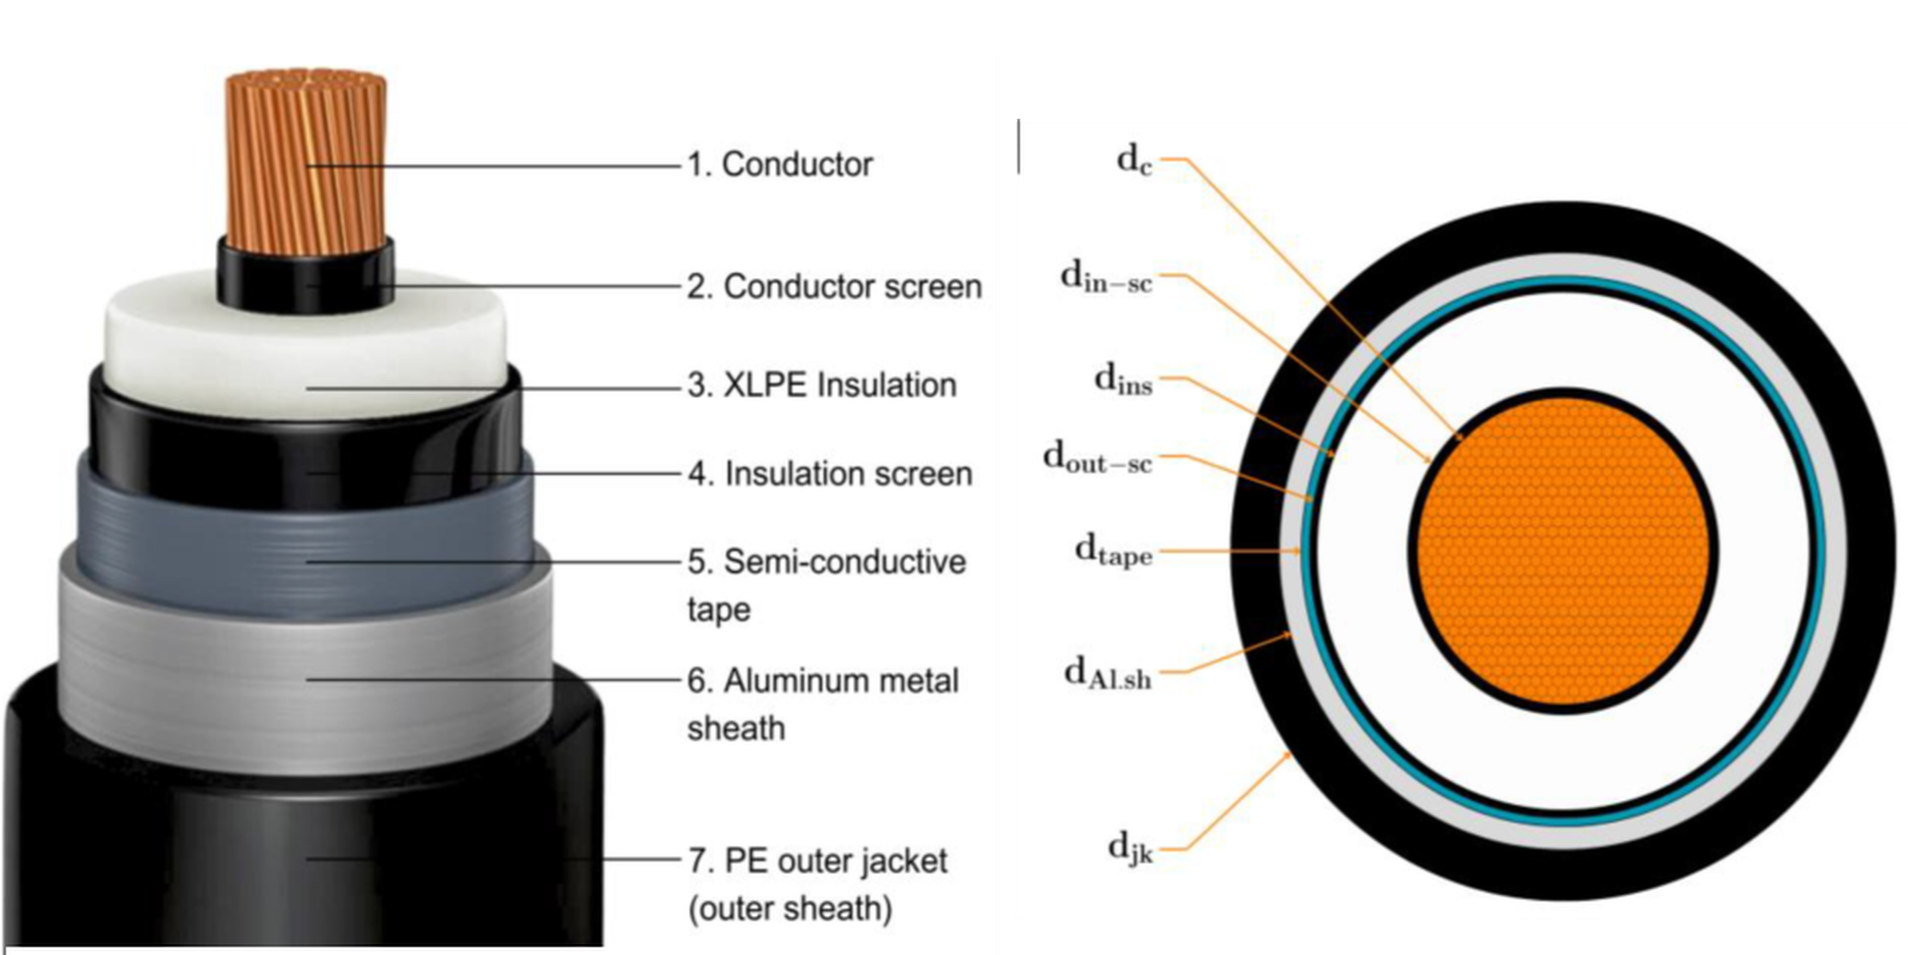
\includegraphics[height=0.27\textheight,keepaspectratio]{kim2025_cable_xsection.png}
\caption[Estructura multicapa de un cable XLPE]{Estructura multicapa de un cable XLPE usado como referencia del objeto de estudio. Fuente: \textcite[fig.~2]{kim2025}.}
\label{fig:cable-multicapa}
\end{figure}

\begin{figure}[htbp]
\centering
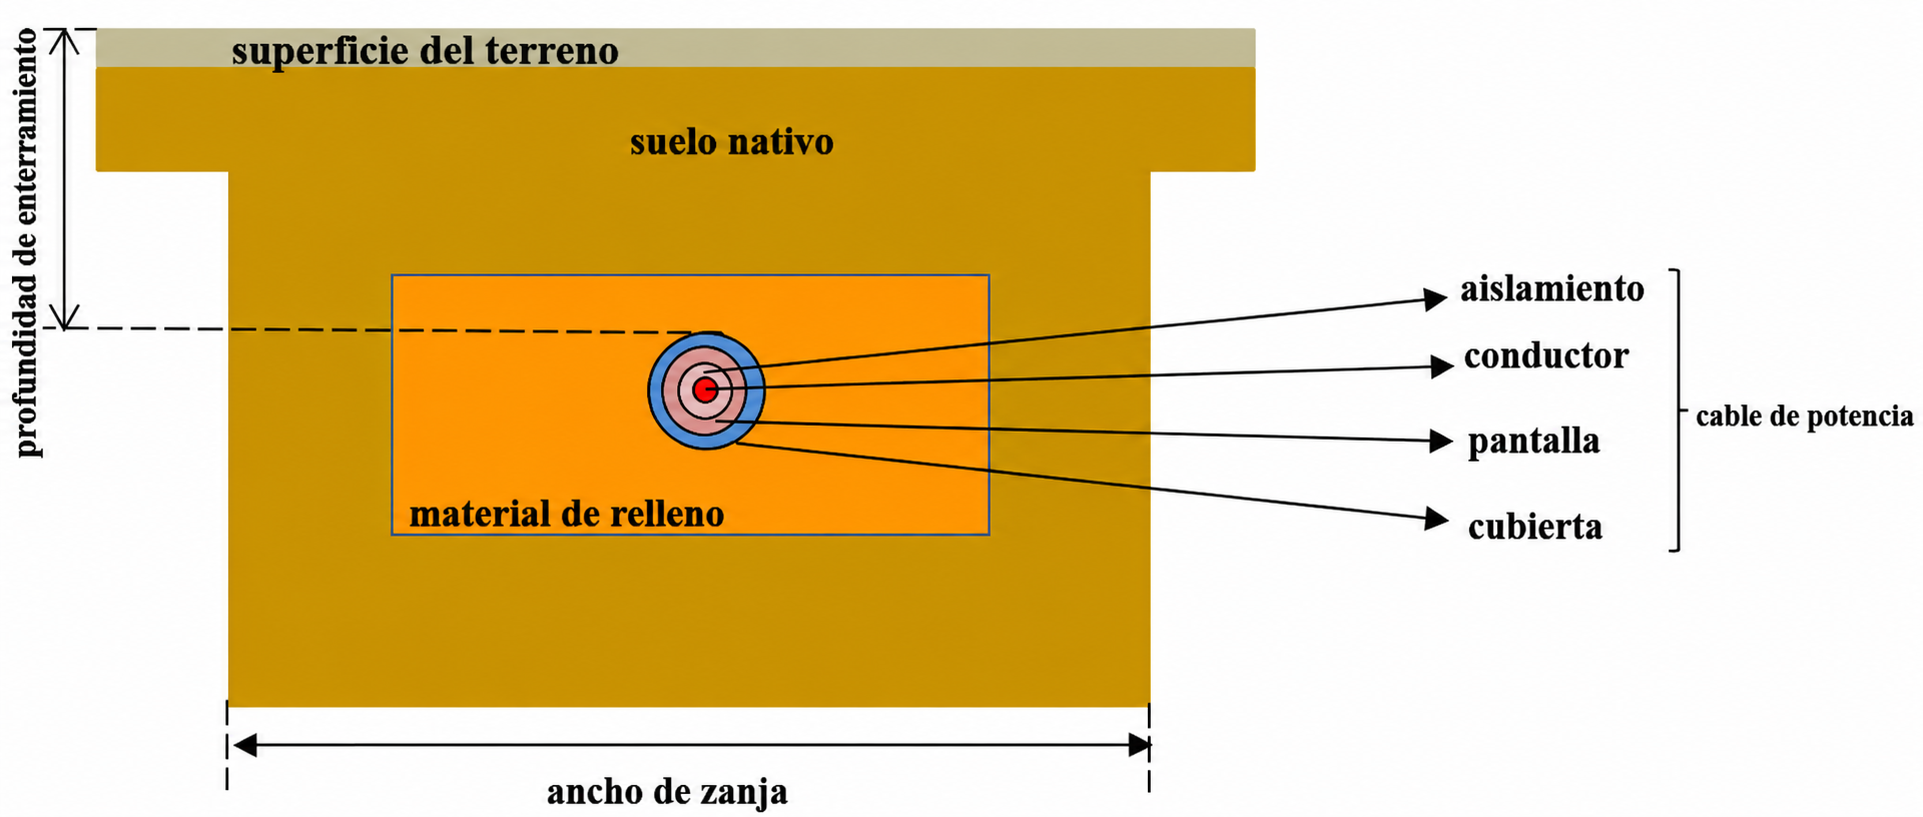
\includegraphics[width=0.96\textwidth,height=6.8cm,keepaspectratio]{enescu_trench_xsection_es.png}
\caption[Zanja y entorno térmico del cable enterrado]{Zanja y entorno térmico del cable enterrado: suelo de relleno, suelo nativo, profundidad de instalación y capas principales del cable. Fuente: Elaboración propia a partir de \textcite[fig.~1]{enescu2021}.}
\label{fig:zanja-cable}
\end{figure}

\subsection{ECUACIÓN DE CONDUCCIÓN Y CONDICIONES AUXILIARES}

En un dominio 2D dependiente del tiempo, la conservación de energía incluye el término de acumulación térmica gobernado por la capacidad térmica volumétrica $\rho(x,y)c_p(x,y)$ (que no debe confundirse con la resistividad térmica $\rhoth$), como expresa la Fórmula~\ref{for:calor-transitorio} \parencites{carslaw1959conduction,kakac2018heatConduction,hahn2012heatConduction}.

\begin{formula}[htbp]
\centering
\begin{equation}
\label{for:calor-transitorio}
\rho(x,y)c_p(x,y)\frac{\partial T(x,y,t)}{\partial t}
=\nabla\!\cdot\!\left(k(x,y)\nabla T(x,y,t)\right)+Q(x,y,t).
\end{equation}
\caption{Ecuación de conducción de calor 2D transitoria. Fuente: Elaboración propia a partir de \textcite{carslaw1959conduction}.}
\end{formula}

Aunque el régimen transitorio resulta relevante en análisis dinámicos bajo ciclos de carga variables \parencites[cláusulas~2--4]{iec60853}[14843--14845]{fariz2026}, esta investigación se acotó al régimen estacionario, en el cual $\partial T/\partial t=0$. Así, el balance térmico se reduce a la Fórmula~\ref{for:calor-estacionario} dentro de cada región material continua $\Omega_i\subset\Omega$ \parencites{carslaw1959conduction,kakac2018heatConduction}[3]{xing2023}.

\begin{formula}[htbp]
\centering
\begin{equation}
\label{for:calor-estacionario}
\nabla\!\cdot\!\left(\kx\nabla T(x,y)\right)+Q(x,y)=0,
\qquad (x,y)\in\Omega.
\end{equation}
\caption{Ecuación de conducción de calor 2D estacionaria. Fuente: Elaboración propia a partir de \textcite{carslaw1959conduction}.}
\end{formula}

Cuando dos materiales distintos entran en contacto perfecto en una interfaz interna $\Gamma_{12}$, se impone la continuidad de temperatura y de flujo normal establecida en la Fórmula~\ref{for:interfaces} \parencites{carslaw1959conduction}{patankar1980numerical}[3]{xing2023}. En los contornos exteriores del dominio se aplican condiciones de Dirichlet, Neumann o Robin según el caso de referencia \parencite[3--5]{enescu2020}.

\begin{formula}[htbp]
\centering
\begin{equation}
\label{for:interfaces}
T_1=T_2,
\qquad
\mathbf{n}\cdot k_1\nabla T_1=\mathbf{n}\cdot k_2\nabla T_2
\quad\text{en }\Gamma_{12}.
\end{equation}
\caption{Condiciones de continuidad térmica en una interfaz. Fuente: Elaboración propia a partir de \textcite{carslaw1959conduction}.}
\end{formula}

La Fórmula~\ref{for:interfaces} garantiza que los cambios de conductividad entre conductor, aislamiento, pantalla, cubierta, relleno y suelo nativo conserven el balance energético sin introducir saltos térmicos no físicos.

\subsection{INTERIOR EXPLÍCITO, ESCALAS Y REPRESENTACIÓN}

Para evitar diferenciar automáticamente funciones indicadoras discontinuas de $k$, el dominio $\Omega$ se particiona en subdominios abiertos $\Omega_i$ con propiedades suaves en su interior. En las capas anulares concéntricas del cable ($a\le r\le b$), la ecuación de calor adopta la forma polar completa de la Fórmula~\ref{for:polar-completa}.

\begin{formula}[htbp]
\centering
\begin{equation}
\rho c_p T_t-\frac{1}{r}\partial_r(rkT_r)-\frac{1}{r^2}\partial_\varphi(kT_\varphi)=Q.
\label{for:polar-completa}
\end{equation}
\caption{Ecuación de calor polar completa en las capas anulares. Fuente: Elaboración propia.}
\end{formula}

La Fórmula~\ref{for:polar-completa} conserva tanto la difusión radial como la angular, pues la proximidad de otros cables o las heterogeneidades del terreno rompen la simetría axisimétrica; el núcleo del conductor ($r=0$) se representa en coordenadas cartesianas normalizadas para preservar la regularidad en el origen. En cada anillo se emplea la coordenada logradial $\eta=\log(r/a)/\log(b/a)$ junto con $\cos\varphi$ y $\sin\varphi$ para ampliar numéricamente capas milimétricas sin alterar su espesor físico ni perder los factores jacobianos al derivar respecto de $(x,y)$. En el suelo se utilizan coordenadas globales normalizadas combinadas con distancias logarítmicas a los ejes de los cables, enfoque emparentado con la normalización multiescala de \textcite{moseley2021fbpinn}. Además, los residuos se adimensionalizan por región mediante escalas locales $T_i^*=q_i^*\ell_i/k_i^*$ y $r_i^*=q_i^*/\ell_i$ para evitar sesgos por área.

\subsection{FUENTE ELÉCTRICA, RESISTENCIA JOULE Y EFECTO PIEL}

La formulación principal compara campos térmicos a fuente volumétrica prescrita, pero incorpora también las ecuaciones del acoplamiento electrotérmico Joule necesario para evaluar pérdidas dependientes de la temperatura y determinar la ampacidad. En el régimen de fuente Joule uniforme por conductor $j$, la resistencia efectiva por unidad de longitud se actualiza linealmente respecto de la temperatura media del conductor $\overline{T}_{c,j}=A_{c,j}^{-1}\int_{\Omega_{c,j}}T\,\mathrm{d}A$, conforme a la Fórmula~\ref{for:joule-resistencia} basada en \textcite{iec60287}.

\begin{formula}[htbp]
\centering
\begin{equation}
\label{for:joule-resistencia}
\begin{aligned}
R_{\mathrm{ef},j}(\overline{T}_{c,j})
&=R_{\mathrm{ef},20,j}\left[1+\alpha_{20,j}
\left(\overline{T}_{c,j}-T_{20}\right)\right],\\
Q_j&=\frac{I_j^2R_{\mathrm{ef},j}(\overline{T}_{c,j})}{A_{c,j}}
\quad\text{en }\Omega_{c,j};\qquad Q=0\quad\text{fuera de los conductores}.
\end{aligned}
\end{equation}
\caption{Resistencia efectiva referida a \SI{20}{\celsius} y fuente Joule uniforme por conductor. Fuente: Elaboración propia a partir de \textcite{iec60287}.}
\end{formula}

En la Fórmula~\ref{for:joule-resistencia}, $T_{20}=\SI{20}{\celsius}$ y $\alpha_{20,j}$ es el coeficiente térmico de resistividad del metal. Cada ficha declara si utiliza resistencia DC documentada ($R_{\mathrm{ef},20}=R_{\mathrm{DC},20}$) o resistencia AC efectiva documentada ($R_{\mathrm{ef},20}=R_{\mathrm{DC},20}(1+y_s+y_p)$), sin aplicar doblemente factores de piel $y_s$ ni proximidad $y_p$.

Para verificar el acoplamiento electrotérmico local en corriente continua (DC) bajo potencial axial común en un conductor largo, la densidad volumétrica de pérdidas se calcula punto a punto a partir de la conductividad eléctrica local $\sigma(T)$ mediante la Fórmula~\ref{for:fuente-dc-local}.

\begin{formula}[htbp]
\centering
\begin{equation}
\sigma(T)=\frac{1}{\rho_{e,0}[1+\alpha(T-T_{e,0})]},\qquad
E_z=\frac{I}{\int_{\Omega_c}\sigma(T)\,dA},\qquad Q=\sigma(T)E_z^2.
\label{for:fuente-dc-local}
\end{equation}
\caption{Fuente Joule DC dependiente de la temperatura local. Fuente: Elaboración propia.}
\end{formula}

Asimismo, para cuantificar la sensibilidad frente a la redistribución radial de la corriente por efecto piel a \SI{60}{\hertz} en un conductor circular macizo aislado, se emplea la solución cilíndrica analítica de Bessel de la Fórmula~\ref{for:piel-volumetrica}, con profundidad de penetración $\delta=\sqrt{\rho_e/(\pi f\mu)}$, $\gamma=(1-\mathrm i)/\delta$ y $z=\gamma a$.

\begin{formula}[htbp]
\centering
\begin{equation}
\frac{R_{\mathrm{AC}}}{R_{\mathrm{DC}}}=\Re\!\left[\frac{zJ_0(z)}{2J_1(z)}\right],\qquad
J_z(r)=\frac{I\gamma J_0(\gamma r)}{2\pi aJ_1(\gamma a)},\quad
Q(r)=\rho_e|J_z(r)|^2.
\label{for:piel-volumetrica}
\end{equation}
\caption{Estimación cilíndrica del efecto piel y su fuente volumétrica. Fuente: Elaboración propia.}
\end{formula}

La integral de $Q(r)$ en la Fórmula~\ref{for:piel-volumetrica} reproduce exactamente la potencia total $I^2R_{\mathrm{AC}}$, lo cual permite aislar el efecto de la distribución espacial radial respecto del aumento neto de pérdidas de corriente alterna. Sin embargo, esta estimación cilíndrica no sustituye un modelo electromagnético completo con proximidad entre fases ni conductores segmentados \parencite{patel2013skin}.

\subsection{CONDUCTIVIDAD, RESISTIVIDAD Y HETEROGENEIDAD}

Mientras la conductividad térmica $k$ cuantifica la facilidad de conducción, las normas y la ingeniería de cables suelen expresar los datos de suelos mediante la resistividad térmica $\rhoth$. En materiales isotrópicos ambas magnitudes son inversas, según la Fórmula~\ref{for:k-rho}, relación empleada sistemáticamente para convertir datos bibliográficos antes de parametrizar el modelo \parencites{farouki1981thermal,devries1966thermal}[secciones~4--6]{ieee442}.

\begin{formula}[htbp]
\centering
\begin{equation}
\label{for:k-rho}
\rhoth=\frac{1}{k},\qquad k=\frac{1}{\rhoth}.
\end{equation}
\caption{Relación entre conductividad y resistividad térmica. Fuente: Elaboración propia.}
\end{formula}

La heterogeneidad térmica del terreno queda parametrizada por el contraste de conductividad $C_k$, el patrón espacial, la extensión $f_h$ de la anomalía y su proximidad $d_h$ respecto al cable. La Tabla~\ref{tab:base-teorica-uso} resume cómo cada magnitud física de estas bases teóricas se traduce en variables operacionales, métricas e interfaces dentro del estudio.

\begin{table}[htbp]
\centering
\caption{Relación entre base teórica y uso metodológico en el estudio. Fuente: Elaboración propia.}
\label{tab:base-teorica-uso}
\begingroup
\footnotesize
\setlength{\tabcolsep}{3pt}
\renewcommand{\arraystretch}{1.22}
\begin{tabularx}{\textwidth}{L{3.2cm}Y Y}
\toprule
\textbf{Base teórica} & \textbf{Relación física} & \textbf{Uso en el estudio} \\
\midrule
Conductividad $\kx$ y resistividad $\rhoth$ & Magnitudes inversas; $k$ gobierna el flujo local según Fourier. & Conversión previa de datos de suelo para construir $P_1$, $E_3$ y $C_4$ (Sección~\ref{sec:dimensiones-operativas}). \\
Campo $T(x,y)$ & Solución de la PDE estacionaria para geometría, fuentes y contornos dados. & Salida continua del artefacto e indicador contenido en VD2--VD4. \\
Temperatura máxima $\Tmax$ & Restricción crítica sobre el aislamiento del conductor. & Indicador de VD2--VD4 y base de $E_T$, $e_{\Tmax}$ y $M_T$ en la Fórmula~\ref{for:metricas-evaluacion}. \\
Ampacidad $\Imax$ & Mayor corriente sostenida que satisface $\Tmax \le T_{\mathrm{lim}}$. & Resultado operativo buscado mediante la condición de la Fórmula~\ref{for:ampacidad}. \\
Interfaces térmicas & Continuidad de temperatura y flujo normal entre materiales. & Requisito físico crítico y criterio explícito de aceptación en la campaña A--D. \\
\bottomrule
\end{tabularx}
\endgroup
\end{table}

\subsection{TEMPERATURA MÁXIMA Y AMPACIDAD}

La ampacidad $\Imax$ corresponde al mayor valor de corriente eficaz $I$ que mantiene la temperatura máxima del conductor por debajo del límite térmico $T_{\mathrm{lim}}$, tal como formaliza la Fórmula~\ref{for:ampacidad} \parencites[3--6]{enescu2021}[cláusulas~4--5]{iec60287}.

\begin{formula}[htbp]
\centering
\begin{equation}
\label{for:ampacidad}
\Imax=\max\left\{I:\max_{(x,y)\in\Omega_c}T(x,y;I)\leq T_{\mathrm{lim}}\right\}.
\end{equation}
\caption{Condición operacional para determinar la ampacidad. Fuente: Elaboración propia.}
\end{formula}

La búsqueda acotada descrita en la Fórmula~\ref{for:ampacidad} resuelve iterativamente el acoplamiento entre temperatura y resistencia $R_{\mathrm{ef}}(T)$ mediante punto fijo relajado. Con ese lazo acoplado, se acota el intervalo $[I_L, I_U]$ mediante bisección hasta cumplir tolerancias geométricas y térmicas comunes en la PINN y en FEM.

\subsection{MÉTODOS DE CÁLCULO TÉRMICO}

Los circuitos térmicos normativos resuelven el sistema mediante resistencias equivalentes y son computacionalmente inmediatos, pero pierden resolución espacial ante entornos heterogéneos \parencite[4--6]{enescu2021}. Los métodos numéricos de campo discretizan el dominio: FEM aproxima por elementos variacionales; las diferencias finitas (FDM) discretizan derivadas sobre mallas estructuradas; y los volúmenes finitos (FVM) integran balances locales sobre celdas de control \parencites{patankar1980numerical}[3--4,93--99]{cigre2025}. Por su parte, las PINN aproximan una solución continua mediante diferenciación automática y optimización de residuos. La Tabla~\ref{tab:metodos-termicos} establece la función complementaria de cada enfoque dentro del estudio.

\begin{table}[htbp]
\centering
\caption{Función de los métodos térmicos dentro de la investigación. Fuente: Elaboración propia a partir de \textcite{iec60287}, \textcite{iec60853}, \textcite{patankar1980numerical}, \textcite[4--6]{enescu2021}, \textcite[3--4,93--99]{cigre2025} y \textcite{raissi2019}.}
\label{tab:metodos-termicos}
\begin{tabularx}{\textwidth}{L{2.8cm}Y Y}
\toprule
\textbf{Método} & \textbf{Fortaleza y límite relevante} & \textbf{Uso en la investigación} \\
\midrule
IEC y circuitos térmicos & Cálculo interpretable mediante resistencias equivalentes; representación espacial limitada. & Línea base normativa cuando coinciden los supuestos de instalación. \\
Analítico o manufacturado & Respuesta exacta conocida y trazable sobre geometrías idealizadas. & Verificación elemental de formulación y operadores del código. \\
FEM & Geometría, capas e interfaces explícitas; exige mallado y estudio de convergencia. & Referencia numérica independiente del campo térmico. \\
FDM & Aproximación directa en grillas regulares; menor flexibilidad en fronteras curvas. & Antecedente comparativo de discretización espacial. \\
FVM & Conservación local de flujos en volúmenes de control; requiere tratamiento de interfaces curvas. & Antecedente numérico de balance energético local. \\
PINN & Aproximación continua con física incorporada; sensible al muestreo y al balance de pérdidas. & Artefacto principal diseñado y evaluado. \\
\bottomrule
\end{tabularx}
\end{table}

\subsection{RED NEURONAL INFORMADA POR FÍSICA}

Una PINN utiliza redes neuronales de propagación hacia adelante (\textit{feed-forward}) de tipo perceptrón multicapa para aproximar la variable física $T_\theta(x,y)$ \parencite[3--4]{xing2023}. Cuando el dominio se descompone por subdominios materiales, cada subregión emplea su propia subred acoplada mediante condiciones de interfaz \parencite[4--6]{shukla2021}. La Figura~\ref{fig:arquitectura-pinn-lawal} ilustra el esquema clásico donde los operadores de diferenciación automática extraen las derivadas espaciales para evaluar el residuo físico.

\begin{figure}[htbp]
\centering
\resizebox{0.94\textwidth}{!}{%
\begin{tikzpicture}[
  font=\small,
  neurona/.style={circle, draw, minimum size=9mm, inner sep=1pt, line width=0.45pt},
  entrada/.style={neurona, fill=lightblue},
  oculta/.style={neurona, fill=lightgray},
  salida/.style={neurona, fill=yellow!55},
  operador/.style={neurona, fill=red!15, minimum size=10.5mm, inner sep=0.5pt,
                   font=\footnotesize, align=center},
  bloque/.style={draw, rounded corners=3pt, align=center, minimum height=10mm,
                 text width=2.35cm, line width=0.45pt},
  grupo/.style={draw=gray!75, fill=lightgray!55, dashed, rounded corners=7pt,
                inner sep=7pt, line width=0.55pt},
  enlace/.style={-{Stealth[length=1.8mm]}, draw=gray!60, line width=0.32pt},
  fisica/.style={-{Stealth[length=2mm]}, draw=gray!75, line width=0.48pt},
  perdida/.style={-{Stealth[length=2.4mm]}, draw=gray!80, dashed, line width=0.9pt}
]
  \node[entrada] (x) at (0,2.1) {$x$};
  \node[entrada] (y) at (0,0.7) {$y$};
  \node[entrada] (t) at (0,-0.7) {$t$};

  \node[oculta] (h11) at (2.25,2.55) {$\sigma$};
  \node[oculta] (h12) at (2.25,1.25) {$\sigma$};
  \node[oculta] (h13) at (2.25,-0.05) {$\sigma$};
  \node[oculta] (h14) at (2.25,-1.35) {$\sigma$};
  \node[oculta] (h21) at (3.75,2.55) {$\sigma$};
  \node[oculta] (h22) at (3.75,1.25) {$\sigma$};
  \node[oculta] (h23) at (3.75,-0.05) {$\sigma$};
  \node[oculta] (h24) at (3.75,-1.35) {$\sigma$};

  \node[salida] (u) at (5.55,1.45) {$u$};
  \node[salida] (v) at (5.55,-0.25) {$v$};

  \node[operador] (id)  at (7.55,2.75) {$I$};
  \node[operador] (dx)  at (7.55,1.40) {$\partial/\partial x$};
  \node[operador] (dy)  at (7.55,0.05) {$\partial/\partial y$};
  \node[operador] (dxx) at (7.55,-1.30) {$\partial^2/\partial x^2$};
  \node[operador] (dyy) at (7.55,-2.65) {$\partial^2/\partial y^2$};
  \node[bloque, fill=yellow!20, text width=1.45cm] (f) at (9.85,0.25) {Residuo\\$f$};

  \node[bloque, fill=yellow!45, text width=3.15cm] (ldata) at (5.30,-3.85)
    {Pérdida de datos\\[0.15em]$\mathcal{L}_{\mathrm{datos}}$};
  \node[bloque, fill=yellow!20, text width=3.15cm] (lphysics) at (10.00,-3.85)
    {Pérdida física\\$\mathcal{L}_{\mathrm{física}}$};
  \node[bloque, fill=lightblue, text width=3.15cm] (ltotal) at (7.65,-5.15)
    {Pérdida total\\$\mathcal{L}_{\mathrm{total}}$};

  \foreach \a in {x,y,t}
    \foreach \b in {h11,h12,h13,h14}
      \draw[enlace] (\a) -- (\b);
  \foreach \a in {h11,h12,h13,h14}
    \foreach \b in {h21,h22,h23,h24}
      \draw[enlace] (\a) -- (\b);
  \foreach \a in {h21,h22,h23,h24}
    \foreach \b in {u,v}
      \draw[enlace] (\a) -- (\b);

  \foreach \a in {u,v}
    \foreach \b in {id,dx,dy,dxx,dyy}
      \draw[fisica] (\a) -- (\b);
  \foreach \a in {id,dx,dy,dxx,dyy}
    \draw[fisica] (\a) -- (f);

  \draw[perdida] (v.south) -- ++(0,-0.40cm) -| (ldata.north);
  \draw[perdida] (f.south) -- (lphysics.north);
  \draw[fisica, line width=0.8pt] (ldata.south) -- (ltotal.west);
  \draw[fisica, line width=0.8pt] (lphysics.south) -- (ltotal.east);

  \begin{scope}[on background layer]
    \node[grupo, fit=(x)(y)(t)] (ginput) {};
    \node[grupo, fit=(h11)(h14)(h21)(h24)] (gred) {};
    \node[grupo, fit=(u)(v)] (gout) {};
    \node[grupo, fit=(id)(dyy)(f)] (gphysics) {};
  \end{scope}
  \node[font=\bfseries\small, above=1mm of gred.north] {Red neuronal};
  \node[font=\bfseries\small, above=1mm of gphysics.north] {Informada por física};
\end{tikzpicture}%
}
\caption[Arquitectura general de una red neuronal informada por física]{Arquitectura general de una red neuronal informada por física: la red aproxima las variables de salida y la diferenciación automática evalúa las derivadas y el residuo de la ecuación gobernante; las pérdidas de datos y física se combinan durante el entrenamiento. Fuente: \textcite[fig.~1]{lawal2022}.}
\label{fig:arquitectura-pinn-lawal}
\end{figure}

Al evaluar la ecuación de calor estacionaria con la aproximación neuronal, se define el residuo físico local $r_f(x,y)$ de la Fórmula~\ref{for:residuo-pinn-calor} sobre puntos de colocación interiores \parencites[686--690]{raissi2019}[1--2,14--17]{lawal2022}.

\begin{formula}[htbp]
\centering
\begin{equation}
\label{for:residuo-pinn-calor}
r_f(x,y)=
\nabla\!\cdot\!\left(k(x,y)\nabla T_\theta(x,y)\right)
+Q(x,y).
\end{equation}
\caption{Residuo físico de una PINN para conducción de calor 2D estacionaria. Fuente: Elaboración propia.}
\end{formula}

Integrando este residuo con las condiciones auxiliares y el balance energético, la función de pérdida lógica del artefacto adopta la forma de la Fórmula~\ref{for:perdida-pinn} \parencites[686--690]{raissi2019}[16]{pan2025}[1--2,17]{lawal2022}. En las campañas principales del estudio se fija $w_d=0$: las temperaturas FEM nunca actúan como etiquetas de entrenamiento, reservándose exclusivamente para la evaluación independiente posterior.

\begin{formula}[htbp]
\centering
\begin{equation}
\label{for:perdida-pinn}
\mathcal{L}(\theta)=
w_f\mathcal{L}_{\mathrm{PDE}}+
w_b\mathcal{L}_{\mathrm{cont}}+
w_i\mathcal{L}_{\mathrm{int}}+
w_d\mathcal{L}_{\mathrm{datos}}+
w_e\mathcal{L}_{\mathrm{energía}}.
\end{equation}
\caption{Función de pérdida lógica del artefacto PINN. Fuente: Elaboración propia a partir de \textcite{raissi2019}.}
\end{formula}

La Figura~\ref{fig:flujo-pinn} organiza el ciclo computacional completo: las coordenadas alimentan la red, la diferenciación automática evalúa los residuos de la PDE, los contornos y las interfaces, y el optimizador actualiza $\theta$ hasta agotar el presupuesto o alcanzar el criterio de parada. La aceptación técnica se verifica posteriormente frente a la referencia FEM y no queda garantizada por la reducción de $\mathcal{L}(\theta)$.

\begin{figure}[htbp]
\centering
\resizebox{0.96\textwidth}{!}{%
\begin{tikzpicture}[
  font=\footnotesize,
  node distance=0.50cm and 0.36cm,
  stage/.style={draw, rounded corners=3pt, align=center, text width=2.30cm,
                minimum height=1.05cm, fill=white, line width=0.45pt},
  model/.style={stage, fill=lightgray},
  residual/.style={stage, fill=lightblue, text width=2.86cm,
                   minimum height=1.55cm},
  total/.style={stage, fill=lightgray, text width=2.62cm,
                minimum height=1.15cm},
  output/.style={stage, text width=2.62cm, minimum height=1.05cm},
  group/.style={draw, dashed, rounded corners=4pt, inner sep=4pt,
                line width=0.4pt},
  arr/.style={-{Stealth[length=2.4mm]}, line width=0.45pt},
  feed/.style={-{Stealth[length=2.4mm]}, line width=0.45pt, dashed,
               rounded corners=2pt}
]
\node[stage] (input) {Entradas\\$(x,y)$; $k,Q$\\contornos/datos};
\node[model, right=of input] (nn) {Red PINN\\capas ocultas\\activación\\$T_\theta(x,y)$};
\node[model, right=of nn] (auto) {Diferenciación\\automática\\$\nabla T_\theta,\nabla\!\cdot(k\nabla T_\theta)$};
\node[residual, right=of auto] (terms) {Pérdidas evaluadas\\[0.15em]
$r_f=\nabla\!\cdot(k\nabla T_\theta)+Q$\\
$r_b,r_i,r_d$};
\node[total, right=of terms] (loss) {Pérdida total\\$\mathcal{L}=\sum_j\lambda_j\mathcal{L}_j$};
\node[output, below=0.62cm of auto] (out) {Salida evaluada\\campo de temperatura\\$T_\theta(x,y)$\\$\Tmax$, punto caliente, $\Imax$};
\node[stage, below=0.62cm of loss] (opt) {Optimizador\\actualiza $\theta$};
\node[group, fit=(terms)(loss), label={[font=\scriptsize]above:Evaluación física y de datos}] (lossbox) {};
\coordinate (fbrail) at ($(out.south)+(0,-0.30cm)$);

\draw[arr] (input) -- (nn);
\draw[arr] (nn) -- (auto);
\draw[arr] (auto) -- (terms);
\draw[arr] (terms) -- (loss);
\draw[arr] (loss) -- (opt);
\draw[feed] (opt.south) |- (fbrail) -| (nn.south);
\draw[arr] (auto.south) -- (out.north);
\end{tikzpicture}%
}
\caption{Flujo lógico de una PINN aplicada a conducción de calor 2D. Fuente: Elaboración propia a partir de \textcite{raissi2019}, \textcite{lawal2022} y \textcite{pan2025}.}
\label{fig:flujo-pinn}
\end{figure}

\subsection{CIENCIA DEL DISEÑO Y NATURALEZA DE LA CONTRIBUCIÓN}

La metodología DSR genera conocimiento prescriptivo mediante el desarrollo y la evaluación rigurosa de artefactos situados \parencite[343--349]{gregor2013}. En esta investigación, el artefacto situado es el prototipo PINN aplicado al arreglo de cables--entorno térmico, mientras que la contribución metodológica abarca la especificación trazable, el protocolo de verificación independiente, el análisis de límites de aplicabilidad y los principios de diseño derivados. Los principios iniciales consisten en conservar la física en cada región, imponer transmisión exacta en interfaces sin promedios inadvertidos, separar verificación numérica de validación experimental, exigir incertidumbre numérica menor que el efecto interpretado y preservar la trazabilidad completa, incluidos los rechazos.

\section{DEFINICIÓN DE TÉRMINOS}
\label{sec:definicion-terminos}

Esta sección precisa los términos técnicos y operacionales utilizados en el documento, indicando las fuentes bibliográficas que los respaldan y las definiciones operacionales delimitadas para el estudio.

\begingroup
\newcounter{terminodefinicion}
\renewcommand*\descriptionlabel[1]{\refstepcounter{terminodefinicion}\normalfont\bfseries\thesection.\theterminodefinicion. #1}
\begin{description}[style=nextline,itemsep=0.5\baselineskip,parsep=0pt,topsep=0.25\baselineskip]
  \item[Ampacidad.] Corriente máxima que puede transportar un cable de forma sostenida sin superar el límite térmico adoptado para sus materiales y condiciones de instalación. Se denota $\Imax$ y se determina buscando la corriente para la cual $\Tmax$ alcanza $T_{\mathrm{lim}}$ \parencites[752--760]{neher1957}{anders2005}[cláusulas~4--5]{iec60287}[3--6]{enescu2021}.

  \item[Ampacidad dinámica (DTR).] Estimación de la capacidad de corriente considerando la evolución temporal de la carga, la temperatura ambiente, el estado del suelo y la inercia térmica previa del cable \parencites[cláusulas~2--4]{iec60853}[3--6]{enescu2021}[14843--14845]{fariz2026}.

  \item[Arreglo de cables--entorno térmico.] Objeto de estudio físico conformado por los cables multicapa, su disposición espacial, el lecho de asiento, el suelo de relleno, el suelo nativo, las fuentes de calor y las condiciones de frontera \parencites[752--760]{neher1957}{anders2005}[3--5]{enescu2020}[4--6]{enescu2021}[1,10,16]{kim2025}.

  \item[Artefacto.] Producto computacional y metodológico diseñado para abordar el problema técnico. Comprende la especificación física, el solucionador PINN, las referencias de verificación, los escenarios de evaluación, las métricas y los principios de diseño derivados \parencites[55--56]{peffers2007}[342--350]{gregor2013}.

  \item[Campo de temperatura.] Distribución espacial estacionaria $T(x,y)$ sobre la sección 2D, a partir de la cual se obtienen $\Tmax$, el punto caliente e $\Imax$. La forma dependiente del tiempo $T(x,y,t)$ corresponde al régimen transitorio \parencites{carslaw1959conduction,kakac2018heatConduction,hahn2012heatConduction}[1,3,16]{pan2025}.

  \item[Caso de referencia (\textit{benchmark}).] Configuración con solución analítica, manufacturada, FEM convergente o resultado publicado empleada como patrón trazable para verificar exactitud y consistencia física \parencites{cigre2022}[93--99]{cigre2025}.

  \item[Ciencia del diseño (DSR).] Paradigma que organiza el diseño, demostración y evaluación de artefactos orientados a problemas prácticos y a la generación de conocimiento prescriptivo \parencites[54--56]{peffers2007}[342--351]{gregor2013}[198--203]{delport2024}.

  \item[Condición de contorno.] Restricción impuesta en la frontera exterior del dominio computacional, expresada como temperatura prescrita, flujo de calor o intercambio convectivo equivalente \parencites{carslaw1959conduction,kakac2018heatConduction}[3--5]{enescu2020}[3--4,93--99]{cigre2025}.

  \item[Conductividad térmica.] Propiedad física $k$, expresada en \si{\watt\per\metre\per\kelvin}, que mide la facilidad de un material para conducir calor. Como campo espacial $\kx$ representa la variación entre el cable, el relleno, el lecho y el suelo nativo \parencites{carslaw1959conduction,kakac2018heatConduction}{farouki1981thermal}[secciones~4--6]{ieee442}.

  \item[Contraste de conductividad.] Relación $C_k$ entre la conductividad de una inclusión heterogénea y la del suelo base circundante \parencites{farouki1981thermal}[1,6--9]{khumalo2025}[1,10,16]{kim2025}.

  \item[Ecuación de conducción de calor.] Ecuación de conservación de energía que vincula conductividad térmica, gradiente de temperatura, fuentes internas y, en régimen transitorio, capacidad térmica volumétrica \parencites{carslaw1959conduction,kakac2018heatConduction,hahn2012heatConduction}[1,3]{xing2023}.

  \item[Ecuación en derivadas parciales (PDE).] Ecuación que relaciona derivadas de una variable física respecto de múltiples coordenadas espaciales o temporales independientes \parencites[686--690]{raissi2019}[1--2]{lawal2022}.

  \item[Extensión de heterogeneidad.] Tamaño geométrico o fracción de área $f_h$ del dominio ocupada por una región con conductividad distinta a la del suelo base \parencites[4--6]{enescu2021}[1,6--9]{khumalo2025}[1,10,16]{kim2025}.

  \item[FEM.] Método de elementos finitos utilizado como referencia numérica independiente sobre mallas conformes refinadas, no como artefacto principal \parencites[4--6]{enescu2021}{patankar1980numerical}[3--4,93--99]{cigre2025}.

  \item[Función de pérdida.] Función objetivo compuesta que minimiza la PINN al combinar residuos de PDE, contornos, interfaces y balance de energía \parencites[686--690]{raissi2019}[16]{pan2025}[1--2,17]{lawal2022}.

  \item[Heterogeneidad térmica.] Variación espacial de la conductividad $\kx$ en el entorno del cable, caracterizada por contraste, patrón geométrico, extensión y proximidad \parencites{farouki1981thermal}[4--6]{enescu2021}[1,6--9]{khumalo2025}[1,10,16]{kim2025}.

  \item[Interfaz térmica.] Frontera interna entre dos materiales contiguos donde se exige continuidad de temperatura y conservación de flujo normal, salvo resistencia de contacto declarada \parencites{carslaw1959conduction}{patankar1980numerical}[3]{xing2023}[3--4,93--99]{cigre2025}.

  \item[Lecho de asiento.] Capa de material colocada inmediatamente debajo del cable en la zanja para soporte mecánico y transferencia de calor hacia el terreno \parencites[1--4]{oclon2015}[1,10,16]{kim2025}[secciones~4--6]{ieee442}.

  \item[Material PAC.] Hormigón de agregado precolocado utilizado como relleno de alta conductividad térmica para mejorar la disipación respecto de la arena natural \parencite[1,10,16]{kim2025}.

  \item[PINN.] Red neuronal informada por física que aproxima el campo térmico mediante una red neuronal y penaliza el incumplimiento de las leyes físicas gobernantes \parencites[686--690]{raissi2019}[1--2,14--17]{lawal2022}[1,3,16]{pan2025}.

  \item[Polietileno reticulado (XLPE).] Material termoestable empleado como aislamiento eléctrico principal en cables de potencia, cuyo límite térmico condiciona la ampacidad \parencites{iec60502_2_2014}[3--5]{enescu2020}[fig.~2]{kim2025}.

  \item[Proximidad de heterogeneidad.] Distancia $d_h$ entre una anomalía térmica del suelo y el cable o zona de generación de calor \parencites[1,6--9]{khumalo2025}[1,10,16]{kim2025}[1--4]{oclon2015}.

  \item[Punto caliente.] Posición espacial donde el campo térmico alcanza la máxima temperatura relevante para la integridad del aislamiento o la operación \parencites[1,6--9]{khumalo2025}[1,10,16]{kim2025}.

  \item[Punto de colocación.] Punto muestreado dentro de los subdominios, contornos o interfaces para evaluar el residuo físico durante el entrenamiento sin requerir etiquetas de referencia \parencites[686--690]{raissi2019}[1--2]{lawal2022}.

  \item[Representación homogénea equivalente.] Sustitución del entorno heterogéneo por una conductividad única ponderada por área $k_{eq}$ empleada como par comparativo frente a la formulación heterogénea \parencites{farouki1981thermal}[4--6]{enescu2021}[3--4,41--42,93--99]{cigre2025}.

  \item[Residuo físico.] Desviación local de la ecuación diferencial gobernante o de una condición auxiliar al evaluar la aproximación neuronal $T_\theta(x,y)$ \parencites[686--690]{raissi2019}[1--2,14--17]{lawal2022}.

  \item[Resistividad térmica.] Propiedad $\rhoth$, expresada en \si{\kelvin\metre\per\watt}, que mide la oposición de un material al paso del calor ($\rhoth=1/k$) \parencites{farouki1981thermal,devries1966thermal}[1,6--9]{khumalo2025}[secciones~4--6]{ieee442}.

  \item[Solución manufacturada.] Solución analítica artificial predefinida que genera términos fuente y condiciones de contorno compatibles para verificar la exactitud del código \parencites{cigre2022}[93--99]{cigre2025}.

  \item[Suelo de relleno.] Material dispuesto dentro de la zanja alrededor de los cables, con propiedades térmicas nativas o mejoradas para favorecer la disipación \parencites{anders2005}[1--3]{atoccsa2024}[1,10,16]{kim2025}[secciones~4--6]{ieee442}.

  \item[Suelo nativo.] Terreno natural circundante a la zanja cuyas propiedades varían según su composición, densidad y contenido de humedad \parencites{farouki1981thermal,devries1966thermal}[1,6--9]{khumalo2025}[secciones~4--6]{ieee442}.

  \item[Temperatura máxima del conductor.] Valor máximo de $T(x,y)$ en la región del conductor, denotado $\Tmax$, que restringe el cálculo de ampacidad \parencites[752--760]{neher1957}{anders2005}[cláusulas~4--5]{iec60287}[3--6]{enescu2021}.

  \item[Validación.] Comprobación mediante evidencia empírica en campo de que el modelo representa una instalación física real; queda fuera del alcance de este estudio \parencites{cigre2022}[93--99]{cigre2025}[350--351]{gregor2013}.

  \item[Verificación.] Evaluación computacional de que la formulación matemática y el código resuelven correctamente el problema especificado frente a soluciones exactas, mallas FEM convergentes y balances energéticos \parencites{cigre2022}[3--4,93--99]{cigre2025}[350--351]{gregor2013}.

  \item[Zona seca.] Región del terreno con pérdida de humedad que incrementa su resistividad térmica local y dificulta la evacuación de calor del cable \parencites[4--6]{enescu2021}[1,6--9]{khumalo2025}[14851--14852]{fariz2026}.
\end{description}
\endgroup

Las bases teóricas y definiciones anteriores delimitan la física del dominio bidimensional estacionario y el marco DSR aplicado. Sobre esta fundamentación, el Capítulo~\ref{ch:propuesta-desarrollo} expone el diseño detallado del artefacto, las etapas experimentales A--D ejecutadas, los resultados obtenidos, su discusión crítica y la estimación de su impacto.
